\documentclass[10pt, letterpaper]{article}
\usepackage{listings}
\usepackage[utf8]{inputenc}
\usepackage{graphicx}
\usepackage{xcolor}
\usepackage{float}
\graphicspath{ {./images/}  }

\definecolor{codegreen}{rgb}{0,0.6,0}
\definecolor{codegray}{rgb}{0.5,0.5,0.5}
\definecolor{codepurple}{rgb}{0.58,0,0.82}
\definecolor{backcolour}{rgb}{0.93,0.95,0.92}

\lstdefinestyle{mystyle}{
    backgroundcolor=\color{backcolour},   
    commentstyle=\color{codegreen},
    keywordstyle=\color{magenta},
    numberstyle=\tiny\color{codegray},
    stringstyle=\color{codepurple},
    basicstyle=\ttfamily\normalsize,
    breakatwhitespace=false,         
    breaklines=true,                 
    captionpos=b,                    
    keepspaces=true,                 
    numbers=left,                    
    numbersep=5pt,                  
    showspaces=false,                
    showstringspaces=false,
    showtabs=false,                  
    tabsize=2
}

\lstset{style=mystyle}

\emergencystretch 5em%
\newcommand{\code}[1]{\texttt{#1}}
\newcommand{\dline}{\par\noindent\rule{\textwidth}{0.2pt}\\}
\usepackage[margin=1in]{geometry}

\title{COMP 421 - Database Systems \\ 
\large Assignment 3: MapReduce and Pig Latin}
\author{Seyed Yazdan Zinati\\seyed.zinati@mail.mcgill.ca\\ 260928077}
\date{\today}

\begin{document}
\maketitle

\section*{Q1}
\subsection*{a}
\begin{tabbing}
    \textbf{Mapper:}\\
    For \= each input key-value pair (linenumber, linetext): \\
    \> Output \= (extract\_browser(linetext), extract\_IP(linetext)) \\
\end{tabbing}

\noindent \textbf{Group and Shuffle} will create for each value of browser (extracted using helper function), a key-value list:
(Browser, ($IP_1$, $IP_2$, ...))

\begin{tabbing}
    \textbf{Reducer:}\\
    For \= each (Browser ($IP_1$, $IP_2$, ...)):\\
    \> result = (browser, count of distinct IP in ($IP_1$, $IP_2$, ...) as num\_users)\\
    \> if num\_users $>$ 100, output result\\
\end{tabbing}

\subsection*{b}
\textbf{Mapper input}: \\
\begin{tiny}
    Line 1: 1.1.2 - frank [10/Oct/2000:13:55:36 -0700] ‘‘GET /apache pb.gif HTTP/1.0’’ 200 2326‘‘http://www.example.com/start.html’’ ‘‘Mozilla/4.08’’\\
    Line 2: 1.1.2 - frank [10/Oct/2000:12:55:36 -0700] ‘‘GET /apache pb.gif HTTP/1.0’’ 200 2326‘‘http://www.example.com/start.html’’ ‘‘Mozilla/4.08’’\\
    Line 3: 1.0.0 - anon [10/Apr/2022:00:55:36 -0700] ‘‘GET /apache pb.gif HTTP/1.0’’ 200 2326‘‘http://www.example.com/start.html’’ Chromium’’\\
    Line 4: 1.0.3 - sophie [10/Apr/2022:00:55:36 -0700] ‘‘GET /apache pb.gif HTTP/1.0’’ 200 2326‘‘http://www.example.com/start.html’’ Chromium’’\\
    Line 4: 1.0.4 - rose [10/Apr/2022:00:55:36 -0700] ‘‘GET /apache pb.gif HTTP/1.0’’ 200 2326‘‘http://www.example.com/start.html’’ Mozilla/4.08\\
    ...\\
    Line N: ...\\
\end{tiny}
Note: IPV4 addresses were shortened for simplicity\\

\noindent \textbf{Mapper output}: (Mozilla/4.08, 1.1.2), (Mozilla/4.08, 1.1.2), (Chromium, 1.0.0), (Chromium, 1.0.3), (Mozilla/4.08, 1.0.4), ...\\

\noindent \textbf{Reducer input}: (Mozilla/4.08, (1.1.2, 1.1.2, 1.1.4, ...)), (Chromium, (1.0.0, 1.0.3, ...))\\

\noindent \textbf{Reducer output}: Assume that firefox (Mozilla) had less than 100 unique IP addresses in this step and Chromium had 1000 unique IP addresses, then the output will be: (Chromium, 1000). We note that there is a duplicate IP in the Mozilla browser tuple which will not be double-counted since we count distinct values.

\subsection*{c}
We can use combine functionality for reducing the network usage and IO. At each mapper, we could perform the same logic as the reducer (counting the number of unique IP addresses). However, contrary to the reducer, we will not filter tuples with less than 100 unique IP addresses as more IP addresses could be added during grouping and shuffling from other mappers. This will reduce network and IO cost since less data will be read and transferred.
\section*{Q2}
\subsection*{a}
We need two pairs of Map/Reduce functions.\\

\begin{tabbing}
    \textbf{Mapper 1:}\\
    For \= each key-value pair (linenumber, linetext):\\
    \> Output (extract\_IP(linetext), extract\_browser(linetext))\\
\end{tabbing}
\textbf{Group and Shuffle} will create for each value of IP (representing users) extracted using provided helper functions a key-value list: (IP, ($Browser_1$, $Browser_2$, ...)).

\begin{tabbing}
    \textbf{Reducer 1:}\\
    For \= each (IP, ($Browser_1$, $Browser_2$, ...)):\\
    \> Output (IP, 1) if count of of distinct values in ($Browser_1$, $Browser_2$, ...) is greater than 1.
\end{tabbing}

\begin{tabbing}
    \textbf{Mapper 2:}\\
    For \= each key-value pair (IP, 1):\\
    \> output (1, IP).
\end{tabbing}
\textbf{Group and Shuffle} will create for each value of 1 (representing users that use multiple broswers) a key-value list: (1, ($IP_1$, $IP_2$, ...)).
\begin{tabbing}
    \textbf{Reducer 2:}\\
    For \= each (1, ($IP_1$, $IP_2$, ...)):\\
    \> Output count of distinct values in list ($IP_1$, $IP_2$, ...).
\end{tabbing}
\textbf{See example of this workflow in Figure 1}

\begin{figure}[H]
    \centering
    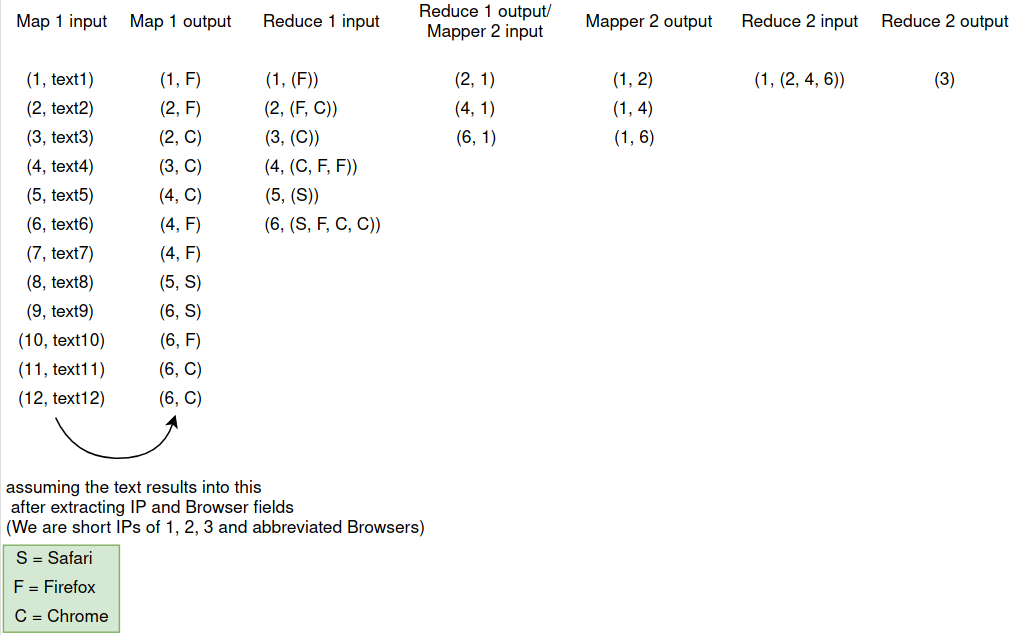
\includegraphics[width=\linewidth]{example}
    \caption{Q2(a) example}
\end{figure}

\subsection*{b}
As can be seen from Figure 1, the designed Map/Reduce workflow only requires 1 reducer process at the second reducer. This is because all tuples have the same key of 1 at the output of the second mapper. As a result, all tuples are grouped into 1 tuple of the following format : (1, ($IP_1$, $IP_2$, ...)). So in this special case, only one reducer process is needed.

\section*{Q6}
What does the schema look like immediately after you perform the GROUP operation step?\\
Each group contains at least one tuple containing the following attributes: country, population, persons fully vaccinated, iso3, iso3, and product name.
\begin{lstlisting}[language=SQL]
grunt> DESCRIBE Grpd;
Grpd: {
    group: chararray,
    Jnd2: {
        (
            Proj::highpop::country: chararray,
            Proj::highpop::population: int,
            Proj::vdatacsv::persons_fully_vaccinated: int,
            Proj::vdatacsv::iso3: chararray,
            vmetacsv::iso3: chararray,
            vmetacsv::product_name: chararray
        )
    }
}
\end{lstlisting}

\end{document}